\chapter{ORP 1 - Substitutivas} \label{ch:orp1subs}
\section*{Questão 1}
\textbf{\cite{Halliday2009}}
\begin{itemize}
    \item[(a)] Se a aceleração máxima que pode ser tolerada pelos passageiros de um metrô é $1,34$ $m/s^2$ e duas estações estão separadas por uma distância de $806$ $m$, qual é a velocidade máxima que o metrô pode alcançar entre as estações?
    \item[(b)] Qual o tempo de percurso?
    \item[(c)] Se o metrô pára por $20$ $s$ em cada estação, qual é a máxima velocidade escalar média do metrô de uma partida à próxima? 
\end{itemize}

\section*{Questão 2}

\textbf{\cite{Halliday2009}} Dois besouros correm em um deserto plano, partindo do mesmo ponto. O besouro 1 corre $0,50$ $m$ para leste e $0,80$ $m$ em uma direção $30^{\circ}$ ao norte do leste. O besouro 2 corre $1,6$ $m$ em uma direção $40^{\circ}$ ao leste do norte e depois corre em outra direção. Quais devem ser (a) o módulo e (b) o sentido da segunda corrida do segundo besouro para que ele termine na mesma posição final que o primeiro besouro?

\section*{Questão 3}

\textbf{\cite{Halliday2009}} Uma bola é lançada a partir do solo. Quando ela atinge ma altura de $9,1$ $m$ sua velocidade é $\vec{v} = (7,6 \hat{i} + 6,1 \hat{j})$ $m/s$, com $\hat{i}$ horizontal e $\hat{j}$ para cima. (a) Qual é a altura máxima atingida pela bola? (b) Qual é a distância horizontal coberta pela bola? Quais são (c) o módulo e (d) o ângulo (abaixo da horizontal) da velocidade da bola no instante em que ala atinge o solo? 

\section*{Questão 4}

\textbf{\cite{Halliday2009}} Na figura abaixo uma bola pe arremessada do alto de um edifício caindo $4,00$ $s$ de uma altura $h = 20,0$ $m$ acima da altura de lançamento. A trajetória da bola no final tem uma inclinação $\theta = 60^{\circ}$ em relação à horizontal. (a) Determine a distância horizontal $d$ coberta pela bola. Quais são (b) o módulo e (c) o ângulo (em relação à horizontal) da velocidade inicial da bola?
\begin{figure}[ht]
\begin{center}
\caption*{Esboço Substituutiva Questão 4.}
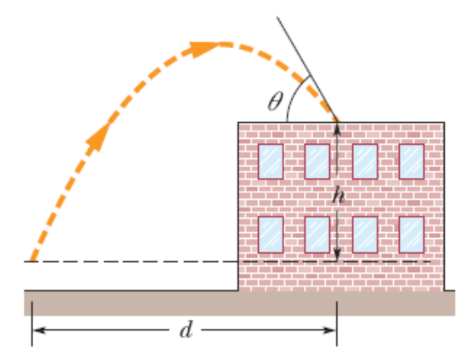
\includegraphics[width=0.4\textwidth]{fig/orp1subs5.png}
\label{fig:ORP1s4}
\caption*{Fonte: \citeonline{Halliday2009}}
\end{center}
\end{figure}

\section*{Questão 5}

\textbf{\cite{Halliday2009}} A figura abaixo mostra uma caixa de massa $m_2 = 1,0$ $kg$ em um plano inclinado sem atrito de ãngulo $\theta = 30^{\circ}$, que está ligada por uma corda, de massa desprezível, a uma outra caixa de massa $m_1 = 3,0$ $kg$ em uma superfície horizontal e sem atrito. A polia não tem atrito e sua massa é desprezível.
\begin{itemize}
    \item[(a)] Se o módulo da força horizontal $\vec{F}$ é $2,3$ $N$, qual é a tração da corda?
    \item[(b)] Qual é o maior valor que o módulo de $\vec{F_2}$ pode ter sem que a corda fique frouxa?
\end{itemize}

\begin{figure}[ht]
\begin{center}
\caption*{Esboço Substituutiva Questão 5.}
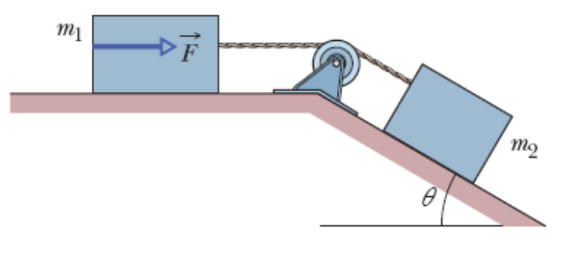
\includegraphics[width=0.4\textwidth]{fig/orp1s5real.png}
\label{fig:ORP1s5}
\caption*{Fonte: \citeonline{Halliday2009}}
\end{center}
\end{figure}

\section*{Questão 6}

\textbf{(\cite{TiplerMosca2006}/Adaptado)} Um bloco de $2,0$ $kg$ é colocado sobre um bloco de $4,0$ $kg$ que está sobre uma mesa sem atrito (ver figura abaixo). Os coefcientes de  atrito entre os blocos são ${\mu}_e = 0,30$ e ${\mu}_c = 0,20$. (a) Qual é a máxima força horizontal $F$ que pode ser aplicada ao bloco de $4,0$ $kg$ se o bloco de $2,0$ $kg$ não deve deslizar? (b) se $F$ tem metade deste valor, encontre a aceleração de cada bloco e a força de atrito atuando sobre cada bloco. (c) Se $F$ tem o dobro do valor encontrado em (a), encontre a aceleração de cada bloco.

\begin{figure}[ht]
\begin{center}
\caption*{Esboço Substituutiva Questão 6.}
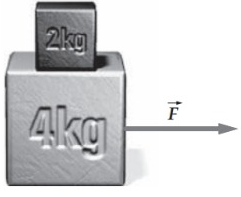
\includegraphics[width=0.4\textwidth]{fig/orp1s6.png}
\label{fig:ORP1s6}
\caption*{Fonte: \citeonline{TiplerMosca2006}}
\end{center}
\end{figure}

\section*{Questão 7}

\textbf{\cite{TiplerMosca2006}} Um bloco de $6,0$ $kg$ escorrega $1,5$ $m$ abaixo sobre um plano inclinado sem atrito que forma um ângulo de $60^{\circ}$ com a horizontal. (a) Desenhe o diagrama de corpo livre para o bloco e encontre o trabalho realizado por cada força, enquanto o bloco escorrega $1n5$ $m$ (medidos ao longo do plano inclinado). (b) Qual é o trabalho total realizado sobre o bloco? (c) Qual é a rapidez do bloco após ter escorregado $1,5$ $m$, se ele parte do repouso? (d) Qual é a sua rapidez, após $1,5$ $m$, se ele parte com uma rapidez inicial de $2,0$ $m/s$?

\section*{Questão 8}

\textbf{\cite{TiplerMosca2006}} Um carrinho de montanha-russa está se movendo com rapidez $v_0$ no início do percurso, quando desce um vale de $5,0$ $m$ e depois sobe até o topo de uma elevação, $4,5$ $m$ acima do início do percurso. Desconsidere o atrito e a resistência do ar. (a) Qual é a menor rapidez $v_0$ necessária para que o carrinho ultrapasse o topo da elevação? (b) Esta rapidez pode ser alterada modificando-se a profundidade do vale, para que o carrinho adquira mais rapidez lá embaixo? Explique.